\section{はじめに}
\label{sec:intro}

%% ---- 背景: 取引データ分析の重要性 ----
小売業・ECサイト・医療など多様な分野において，取引データの蓄積と分析は意思決定の
基盤となっている．取引データに対するパターンマイニングの中でも，
特定の期間内に頻繁に出現するアイテムセットを抽出する「密集パターン」の検出は，
季節性・プロモーション効果・社会的トレンドといった一時的な要因を特定する
手がかりを与える点で重要性が高い．

%% ---- DSAA2025 の問題設定を簡潔に引用 ----
従来の頻出アイテムセットマイニング手法（Apriori\cite{agrawal1994fast}，
FP-Growth\cite{han2000mining}，ECLAT\cite{zaki1997new}）は，
データ全体に渡るグローバルな出現頻度を評価するため，特定期間への密集を
捉えることができない．この限界を克服するために，スライディングウィンドウ機構を
用いて密集区間を完全列挙する手法 Apriori-window \cite{dsaa2025} が提案されている．
Apriori-window は固定ウィンドウを時系列方向にスライドしながらアイテムセットの
局所出現頻度を計算し，密集区間を網羅的に抽出する厳密解法である．

%% ---- バスケット構造の現実的な存在 ----
しかし，現実の取引データには Apriori-window が暗黙的に仮定する
「1 トランザクション = 1 購買イベント」という構造が成立しないケースが多い．
例えば，小売店では同一日付に複数の顧客が独立して商品を購入する．
オンラインマーケットプレイスでは，1 日に同じ配達先への複数の注文が
1 つの集約レコードとして記録されることがある．
これらの場合，1 トランザクション（時間帯）内に複数の独立した購買イベント，
すなわち複数の \emph{バスケット} が混在する．

%% ---- 偽共起の具体例 ----
\begin{figure}[t]
    \centering
    % ユーザー作成予定: 偽共起の動機付け例（詳細は本文末の図案を参照）
    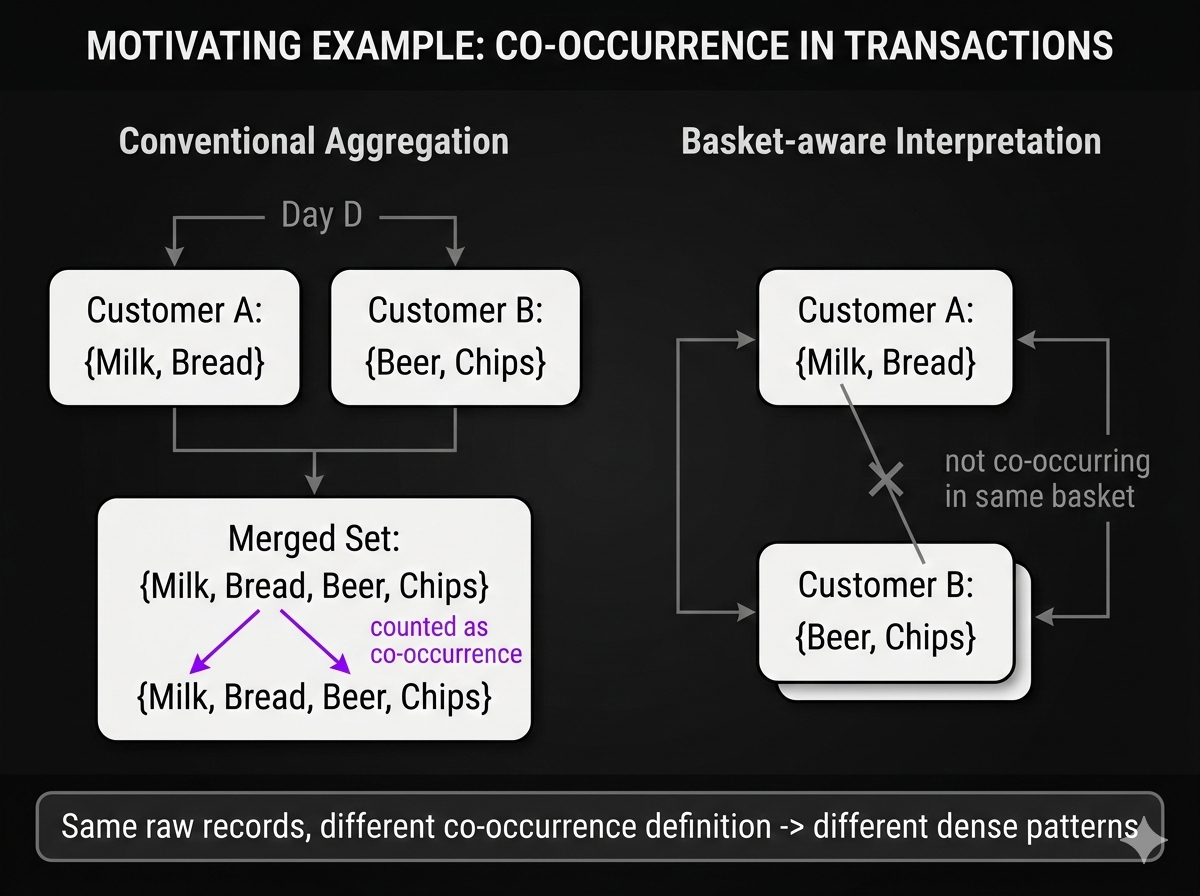
\includegraphics[width=\linewidth]{fig/motivating_example.pdf}
    \caption{偽共起の発生メカニズム．同一日に顧客 A が
    \{牛乳，パン\}，顧客 B が \{ビール，ポテチ\} を購入した場合，
    従来法（左）はこれらを統合して \{牛乳，パン，ビール，ポテチ\} とみなし，
    (牛乳, ビール) を共起として記録する（偽共起）．
    提案手法（右）はバスケットを独立に扱うため，(牛乳, ビール) を
    共起とは判定しない．}
    \label{fig:motivating}
\end{figure}

図~\ref{fig:motivating} に偽共起の典型例を示す．
ある小売店において月曜日に顧客 A が \{牛乳, パン\} を，
顧客 B が \{ビール, ポテチ\} を独立に購入したとする．
このデータを「日付単位のトランザクション」として集約する従来法では，
月曜日のトランザクションは \{牛乳, パン, ビール, ポテチ\} という
単一アイテムセットになる．
その結果，(牛乳, ビール) は「月曜日に共起した」とカウントされる．
同じパターンが木曜日や金曜日にも繰り返せば，(牛乳, ビール) は
高頻度パターンとして抽出されてしまう．
しかし実際には，牛乳とビールは一度も同一の購買かごに入ったことがなく，
この「共起」は統計的な人工物——すなわち \emph{偽共起}——に過ぎない．

%% ---- 問題の定式化 ----
この問題の根本原因は，複数の独立した購買イベントが
1 つのトランザクションに集約される際に，
バスケット間のアイテムが区別なく混合されることにある．
従来の Apriori-window は，各トランザクションが単一のアイテムセットを
もつという仮定のもとで設計されているため，この種の偽共起を
原理的に排除できない．

偽共起の問題は，ファルス・ポジティブ（実際には無関係のアイテム対を
「関連あり」と誤検知すること）として解釈できる．
これにより，マーケティング戦略や棚割り最適化など，
パターンマイニングの下流応用において誤った意思決定が引き起こされる
リスクがある．

%% ---- 提案手法の概要と主貢献 ----
本稿では，バスケット構造を明示的に扱う拡張手法 \emph{Basket-aware Apriori-Window}
（以降 Phase 1 と呼ぶ）を提案する．本稿の主貢献は以下の通りである．

\begin{itemize}
    \item \textbf{問題の定式化}: バスケット構造付きトランザクションデータにおける
    偽共起を厳密に定義し，偽共起パターン率 (SPR: Spurious Pattern Rate) を
    評価指標として提案する（第~\ref{sec:problem_def}節）．

    \item \textbf{提案アルゴリズム}: 共起の定義をバスケット内共起に限定した
    Basket-aware Apriori-Window を設計し，SPR = 0 を原理的に保証する
    （第~\ref{sec:proposed_method}節）．

    \item \textbf{理論的保証}: バスケット内共起においても Apriori の反単調性が
    成立することを証明し，効率的な候補生成を正当化する
    （第~\ref{sec:proposed_method}節）．

    \item \textbf{実験的検証}: 合成データ実験により，$\lambda_{\text{baskets}}$ の
    増加に伴って従来法の SPR が単調増加する一方，
    提案手法は SPR = 0 を維持することを実証的に確認する
    （第~\ref{sec:experiments}節，現在準備中）．
\end{itemize}

%% ---- 論文構成の案内 ----
本稿の構成は以下の通りである．
第~\ref{sec:related_works}節で関連研究を概観する．
第~\ref{sec:problem_def}節でバスケット構造付きトランザクションデータの
形式的定義と解くべき問題を述べる．
第~\ref{sec:proposed_method}節で提案手法 Phase 1 のアルゴリズムと
その理論的性質を説明する．
第~\ref{sec:experiments}節で合成・実データを用いた実験結果を報告し，
第~\ref{sec:conclusion}節でまとめと今後の課題を述べる．
